% ----------------------------------------------------------------------------------------------------------
% Eigene Projektbeschreibung und -ergebnisse
% ----------------------------------------------------------------------------------------------------------
\section{Hauptteil - Projektbeschreibung und Projektergebnisse}\label{ergebnisse}
Der Hauptteil soll damit beginnen, die Grundlagen des Lösungsansatzes zu erläutern. Dazu werden zuerst die Mathematischen Grundlagen aufgezeigt. Danach werden die verwendeten selbst erstellten Algorithmen besprochen. Da dabei gewisse Bibliotheken mit Python zum Einsatz kamen, sollen diese im ersten Schritt kurz erwähnt werden. Der finale Software-Aufbau wird vollständig in einem späteren Kapitel vorgestellt.
	
	\subsection{Bibliotheken}
	Der Lasertriangulationssensor wurde vor Allem mit OpenCv und ROS2 entwickelt. OpenCv bietet die perfekte Unterstützung für die benötigte Bildverarbeitung. Diverse Funktionen, um Bilder zu bearbeiten, zur Kamerakalibrierung und zum Errechnen der Ebenengleichung sind in OpenCv implementiert.
	ROS2 kümmert sich um die Automatisierung und den generellen Ablauf eines Scanvorgangs. In der Forschung und Entwicklungs-Projekt mit RINNTECH wird zusätzlich auch ROS2 als übergeordnetes System genutzt. Deshalb war ROS2 auch eine Anforderung an das Projekt. Die vorher benutzte RGB-D-Kamera Intel RealSense ist ebenfalls in der Lage über ROS2 angesprochen zu werden. Da der OpenSource-Lasertriangulationssensor diese ersetzten soll, ist die Verwendung von ROS2 ein logischer Schritt.
	
	\subsection{Der Grundlegende Aufbau}
	Der grundlegende Aufbau orientiert sich an den Lösungsansatz. Notwendig sind dafür nur ein Linienlaser und eine Kamera. Zuerst wurde für einen Prototyp zum Testen eine Webcam verwenden, später eine Industriekamera. Auschlaggebend zum Funktionieren des theoretischen Lösungsansatz ist, dass die Kamera einen Linienversatz aufnehmen kann. Um das zu erreichen werden Kamera und Laser in einem gewissen Winkel zueinander gesetzt. Durch die Perspektive der Kamera entsteht der Linienversatz. Dabei ist egal, ob die Kamera von oben auf das Objekt zeigt und der Laser schräg sitzt oder andersrum. Die Lasertriangulationssensoren aus der Industrie weisen zumeist den Aufbau aus Abb. 1 auf.
	
	\begin{figure}[h]
		\centering
		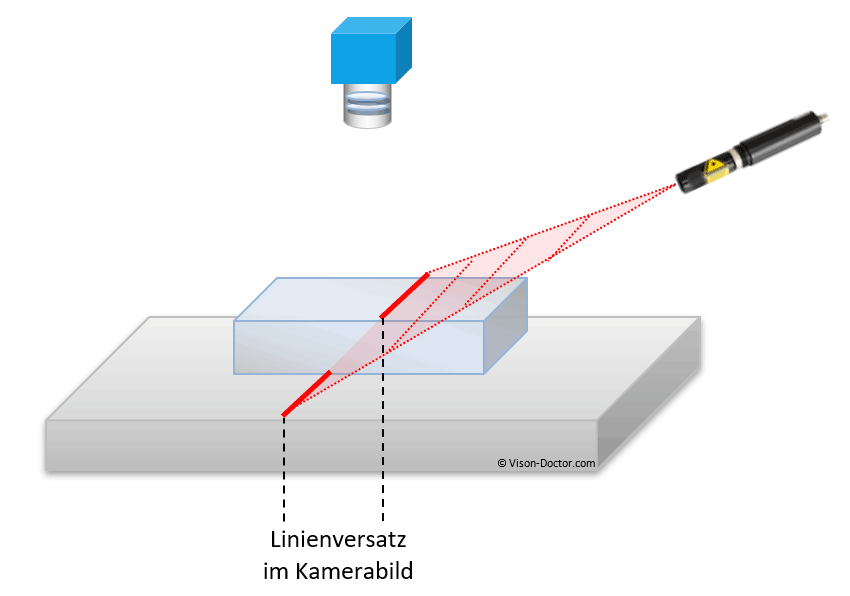
\includegraphics[height=10cm]{img/grundlagen/lasertriangulation_2}
		\caption{Positionen bei der Lasertriangulation}
		\label{lasertriangulation}
	\end{figure}
	
	Der erste Schritt in der Erarbeitung des Sensors war es, die Möglichkeit zu entwickeln, eine aufgenommene Laserlinie in eine korrekte Punktewolke umzusetzen. Danach muss es ermöglicht werden den Sensor über bzw. das Objekt unter dem Sensor bewegen zu können. Mehr zu dem genauen Aufbau des fertigen 3D-Scanner wird im Kapitel \ref{chap:aufbau_hardware} Aufbau / Hardware erläutert. Für die folgenden Erklärungen zur mathematischen Grundlage, Bildverarbeitung und Kalibrierung ist nur wichtig zu wissen, dass die Kamera und Laser in einem Winkel zueinander über dem Objekt angebracht sind. 
	
	\subsection{OpenCv Pinhole Camera Model}
	Der Anfang aller Berechnungen des Lasertriangulationssensors ist immer ein Bild. Die Kamera als optischer Sensor ist die einzige Informations-Quelle. Ein Bild besteht aus Pixeln. Diese sind 2-Dimensional. Es muss also eine Möglichkeit gebunden werden, die dritte Dimension zu finden. Für die gesuchten 3D-Punkte des Objektes ist dafür eine Ebenen-Gleichung für die Laser-Ebene notwendig. Diese ist nicht von Anfang an bekannt und es gilt, diese herauszufinden. Trotzdem wird nach einem Vorgehen gesucht, welches nur aus dem Bild und mithilfe der Kamera 3D-Informationen liefern kann. Genau diese Informationen sind zugänglich mit den Pinhole Camera Model von OpenCv. In OpenCv ist eine Kamera genauso, wie eine Lochkamera begriffen.
	
	\begin{figure}[h]
		\centering
		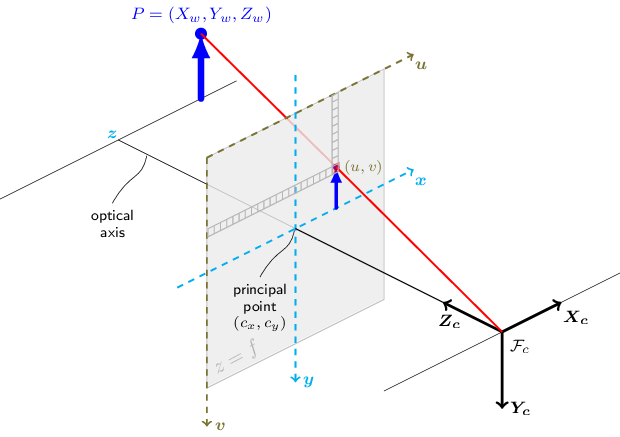
\includegraphics[width=0.7\linewidth]{img/grundlagen/pinhole_camera_model.png}
		\caption[test]{Pinhole Camera Model}
		\captionsource{tesaugdsakif sd}
		\label{fig:pinhole-camera-model}
	\end{figure}

	In Abb. 2 ist dieses Modell dargestellt. Dabei gilt  als optisches Zentrum, welches bei einer Lochkamera das Lochblende ist. Daran orientiert sich das Kamera-Koordinatensystem. Bei einer Lochkamera ist es üblich, dass eine Szene aus der Echten Welt aufgenommen wird. Diese wird über die Öffnung auf dem Kopf gespiegelt auf einem Schirm abgebildet.
	
	
	
	Zum Vergleich ist in Abb. \ref{fig:pinhole-camera-model} das Modell einer Lochkamera zu sehen. Wenn man die beiden Darstellungen vergleicht, fällt auf, dass der „Schirm“, auf dem das Bild als Reflektion dargestellt wird bei der Lochkamera hinter der Lochblende ist und bei dem Modell von OpenCv davor. Die physikalisch korrekte Darstellung ist die der Lochkamera. Jedoch ist OpenCv nicht auf die richtige physikalische Darstellung angewiesen. Mathematisch macht es keinen Unterschied, ob die Bild-Ebene vor oder hinter dem optischen Zentrum ist. So kann ein Punkt in der Szene als Vektor begriffen werden, der durch die Bild-Ebene einen Pixel definiert und zum optischen Zentrum führt. Zu sehen in Abb.2 als die rote Linie. In unserem Fall kennen wir das Bild und die genaue Position eines Pixels mit u und v. Das Ziel ist es 3D-Koordinate zu erhalten.
	
	\subsection{Mathematische Grundlage}
	Grundlegend für die Umrechnung des Pixels in der Bild-Ebene als Vektor mit u und v zu der 3D-Koordinate ist die folgende Formel:
	
	\begin{equation}
		s \; p_{pix} = A \begin{bmatrix} R|t \end{bmatrix} p_w
		\label{eq:basic_trans}
	\end{equation}
	
	Hierbei ist \( p \) der Pixel im Bild. \( Pw \) ist die 3D-Koordinate, welche gesucht wird. \( A \) ist die Kamera-Matrix und \( \begin{bmatrix} R|t \end{bmatrix} \) die Rotation und Translation vom Kamerakoordinatensystem zum Weltkoordinatensystem. Kamera-Matrix, Rotation und Translation sind hierbei neu. Die genaue Bedeutung wird in dem Kapitel \ref{chap:kalibierung} Kalibrierung genannt. Zum Verstehen der Formel ist hier nur wichtig, dass diese durch eine Kamerakalibrierung herausgefunden werden können. Die Variablen sind also bekannt. Kamera-Matrix und Rotation sind beide jeweils 3x3 Matrizen. Die Translation wird durch einen Vektor (3x1) beschrieben. 
	
	\begin{equation}
		s \; \begin{bmatrix}
		u \\ 
		v \\ 
		1
		\end{bmatrix} = \begin{bmatrix}
		f_x & 0 & c_x \\
		0 & f_y & c_y \\
		0 & 0 & 1
		\end{bmatrix} \begin{bmatrix}
		r_{11} & r_{12} & r_{13} & t_1 \\ 
		r_{21} & r_{22} & r_{23} & t_2 \\ 
		r_{31} & r_{32} & r_{33} & t_3 \\
		0 & 0 & 0 & 1
		\end{bmatrix} \times \begin{bmatrix}
		X \\ 
		Y \\ 
		Z \\
		1
		\end{bmatrix}
		\label{eq:basic_trans_complete}
	\end{equation}
	
	In der Formel (\ref{eq:basic_trans_complete}) wird dies noch einmal genauer gezeigt. Bekannt sind also \( p \), \( A \) und \( \begin{bmatrix} R|t \end{bmatrix} \). Unbekannte Variablen sind \( s \) der Scale-Factor und \( p_w \) die Weltkoordinate.
	
		\subsubsection{Homogene Koordinaten}
		In der Formel (\ref{eq:basic_trans_complete}) sind die Rotation (\( R \)), die Translation (\( t \)) als homogenen Matrix und  der Punkt im Weltkoordinatensystem (\( p_w \)) als homogener Vektor dargestellt. Der Vorteil vom Verwenden einer homogenen Matrix ist, dass beliebig viele Transformationen im dreidimensionalen Raum in dieser zusammengefasst werden können. Die Matrix kann dann auf einen Punkt im dreidimensionalen Raum, dargestellt als homogener Vektor, angewandt werden. In diesem Fall sind die Transformationen eine Rotation und eine Translation von dem Punkt im Weltkoordinatensystem zu dem Kamerakoordinatensystem. Das Zusammenführen von Rotation und Translation ergibt Sinn. Die Transformation von dem einen Koordinatensystem in das andere ist nur abgeschlossen, wenn sowohl die Rotation als auch die Translation auf den Zielvektor angewandt wurden. Die Formel (\ref{eq:basic_trans}) soll aber im Folgendem nach dem Punkt im Weltkoordinatensystem umgestellt werden (siehe (\ref{eq:pixel_zu_welt})). Für diese Umstellung wird die homogene Matrix wieder aufgeteilt. Damit dieser Vorgang keine nachvollziehbar ist soll kurz die Entstehung der homogenen Matrix für dieses Beispiel erläutert werden.
		
		Die grundsätzliche Transformation (Rotation + Translation), die angewandt werden soll ist:
		
		\begin{equation}
			\begin{aligned}
				v' &= R \; v + t \\
				&= \begin{pmatrix}
				r_{11} & r_{12} & r_{13} \\ 
				r_{21} & r_{22} & r_{23} \\ 
				r_{31} & r_{32} & r_{33}
				\end{pmatrix} v + \begin{pmatrix}
				t_1 \\ t_2 \\ t_3
				\end{pmatrix}
			\end{aligned}
		\label{eq:rot_trans}
		\end{equation}
		
		Dabei ist v ein Beispielvektor.
		
		Eine homogene Matrix ist eine 4x4-Matrix. Die unterste Zeile ist immer (0, 0, 0, 1). Beide Transformationen können in ihr eingebunden werden. Die Matrix wird dann mit den homogenen Vektor verrechnet:
		
		\begin{equation}
			\begin{aligned}
				v'_{homogen} &= \begin{pmatrix}
				r_{11} & r_{12} & r_{13} & t_1 \\
				r_{21} & r_{22} & r_{23} & t_2 \\
				r_{31} & r_{32} & r_{33} & t_3 \\
				0 & 0 & 0 & 1
				\end{pmatrix} \times \begin{pmatrix}
				v_1 \\
				v_2 \\
				v_3 \\
				1
				\end{pmatrix} \\
				&= \begin{bmatrix}
				R|t
				\end{bmatrix} v_{homogen}
			\end{aligned}
		\label{eq:rot_trans_homgen}
		\end{equation}
		
		\subsubsection{Transformationen}
		Die Grundlegende Formel soll jetzt umgestellt werden, um den 3D-Punkt im Weltkoordinatensystem anhand eines Pixels zu errechnen. Die angewandten Transformationen werden durch die folgende Abbildung noch einmal verdeutlicht.
		
		\begin{figure}[h]
			\centering
			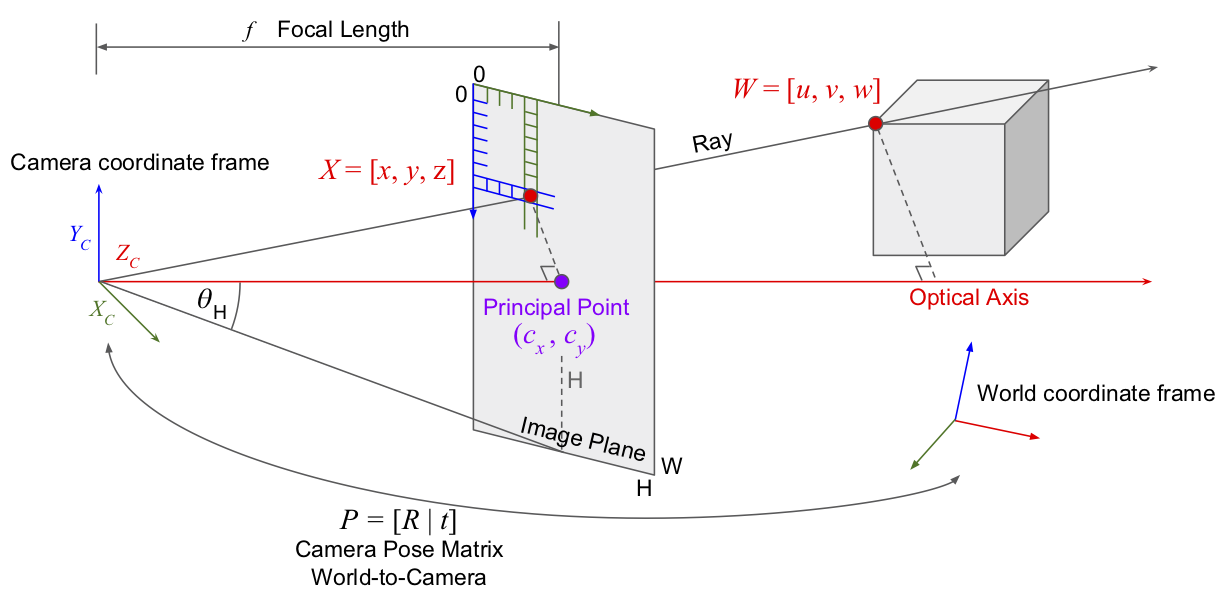
\includegraphics[width=0.9\linewidth]{img/grundlagen/pinhole_camera_model_2.png}
			\caption[Transformationen]{Transformationen im Pinhole Camera Model}
			\captionsource{https://www.oreilly.com/library/view/mastering-opencv-4/9781789533576/848e4e77-32ec-499d-9945-cb0352e28236.xhtml}
			\label{fig:pinhole-camera-model_transformations}
		\end{figure}
		
		Das Ziel ist es den 3D-Punkt im Weltkoordinatensystem zu errechnen. Die Rotation (R) und Translation (t) werde für die Umrechnung in das Kamerakoordinatensystem benötigt. Das sind die sogenannten extrinsischen Parameter. Die Kamera-Matrix beschreibt die Transformation zur Bild-Ebene bzw. den Pixel-Koordinaten-System. Die Matrix enthält die sogenannten intrinsischen Parameter. Wir können einen Pixel im Bild auswählen und mithilfe dieser Parameter den entsprechenden Punkt im Weltkoordinatensystem errechnen.
		
		\begin{equation}
			\begin{aligned}
				 \begin{bmatrix} A \end{bmatrix} \begin{bmatrix} R|t \end{bmatrix} p_w &= s \; p_{pix} \\
				 \begin{bmatrix} R|t \end{bmatrix} p_w &= s \begin{bmatrix} A \end{bmatrix}^{-1} p_{pix} \\
				 \begin{bmatrix} R \end{bmatrix} p_w &= s \begin{bmatrix} A \end{bmatrix}^{-1} p_{pix} - t \\
				 p_w &= s \begin{bmatrix} R \end{bmatrix}^{-1} \begin{bmatrix} A \end{bmatrix}^{-1} p_{pix} - \begin{bmatrix} R \end{bmatrix}^{-1} t \\
				 p_w &= s \; \vec{a} - \vec{b} \\
				 wobei: \quad \vec{a} & = \begin{bmatrix} R \end{bmatrix}^{-1} \begin{bmatrix} A \end{bmatrix}^{-1} p_{pix} \\
				 \vec{b} &= \begin{bmatrix} R \end{bmatrix}^{-1} t
			\end{aligned}
			\label{eq:pixel_zu_welt}
		\end{equation}
		
		Diese Gleichung ist die Grundlage der Errechnung von 3D-Informationen. \( \vec{a} \) und \( \vec{b} \) dienen zur Vereinfachung. Wenn \( \begin{bmatrix} R \end{bmatrix} \), \( \begin{bmatrix} A \end{bmatrix}^{-1} \) und \( p_{pix} \) miteinander verrechnet werden entsteht ein Vektor (\( \vec{a} \)). Dasselbe gilt für \( \begin{bmatrix} R \end{bmatrix}^{-1} \) und \( t \) (\( \vec{b} \)). \newline
		Der neue Ausgangspunkt ist die errechnete Weltkoordinate. Nach Aufgabenstellung sollen errechnete Koordinaten immer aus Sicht der Kamera dargestellt werden. Dazu wird die folgende Transformation benötigt. 
		
		Weltkoordinate zu Kamerakoordinate:
		
		\begin{equation}
			p_{cam} = \begin{bmatrix} R \end{bmatrix} \; p_w + t
			\label{eq:welt_zu_kamera}
		\end{equation}
		
		Kamerakoordinate zur Weltkoordinate:
		
		\begin{equation}
			p_w = \begin{bmatrix} R \end{bmatrix}^{-1} \; (p_{cam} - t)
			\label{eq:kamera_zu_welt}
		\end{equation}
		
		Anzumerken ist noch, das \( s \) der Scale-Factor immer noch eine Unbekannte ist. Es scheint also, als ob die Gleichung (\ref{eq:pixel_zu_welt}) noch nicht lösbar sei. Sobald konkrete Werte ausgerechnet werden sollen, muss \( s \) bekannt sein. Das passiert zum ersten Mal beim Erstellen der Ebenengleichung für die Laser-Ebene bei der extrinsischen Kalibrierung. Dabei wird auch darauf eingegangen, wie \( s \) errechnet werden kann.  
	\subsection{Bildverarbeitung}
	Bekannt sind nun gewisse Grundlagen, wie wir mit einem ausgewählten Pixel im Bild umgehen können. Die Rechnungen und Transformationen sollen aber nicht auf zufällige oder sogar alle Pixel im Bild angewandt werden. Sie sollen auf ganz bestimmte ausgewählte Pixel erfolgen. Und zwar ganz genau diese, die zur abgebildeten Laserlinie gehören. Die Laserlinie ist immer unser Ausgangspunkt für die 3D-Informationen. Alle anderen Pixel interessieren uns im Grunde nicht. Oder anders; die Pixel, die wir brauchen, sind die, die die Laserlinie abbilden. \newline
	Pixel können einfach und eindeutig als Tupel benannt werden. Sie können als Punkt in einem zweidimensionalen Koordinatensystem begriffen und dann mit einem horizontalen und vertikalen Wert genau gekennzeichnet werden. Benötigte wird eine Menge an diesen Tupeln, für die gilt, dass sie teil der Laserlinie im Bild sind. Mit diversen Methoden der Bildverarbeitung also jene Pixel herausgefunden und abgespeichert, um mit ihnen weiterarbeiten zu können. Das folgende Kapitel bildet somit einen Algorithmus ab, dessen Ziel es ist ein Bild entgegen zu nehmen und die Pixel der Laserlinie zurückzugeben. 
	
		\subsubsection{Das Erkennen der Laserlinie}
		Der erste Schritt des Algorithmus muss sein, die Laserlinie im Bild zu erkennen. Am Anfang des Praktikums bin ich hier experimentell vorgegangen. Das bedeutet, dass ich mir ein Lösungsansatz des Problems ausgedacht und diesen mit einen einfachen Python-Script geprobt habe. Danach habe ich diesen kurz evaluiert und die aufgekommenen Probleme zusammengefasst. Der nächste Schritt war dann, nach einer anderen Methode zu suchen, die weniger Probleme oder auch höhere Genauigkeit aufweist. Dabei war ein wichtiges Kriterium die Genauigkeit der ausgewählten Pixel. Jeder Pixel, der vom Algorithmus markiert wird, aber nicht zur eigentlichen Laserlinie gehört wird in einem Fehler in der am Ende erstellten Punktewolke enden. Es wird also ein Punkt im Raum gezeigt, der nicht zur eingescannten Oberfläche passt. Dieser hängt dann beispielsweise in der Luft bzw. ist an einer Stelle im Koordinatensystem wo sich eigentlich nichts befindet. Dieses sogenannte Rauschen soll möglichst gering sein. Getestet habe ich das, indem ich mit den ausgewählten Pixeln eine Bitmaske erstellt und ein Binärbild erstellt. Vorliegen hatte ich dann also ein Bild in dem alle Pixel schwarz sind außer die der durch die Maske getroffene Pixel. Diese sind dann weiß. Die Laserlinie soll also in weiß gut sichtbar sein. Alle Pixel die auch weiß sind, aber offensichtlich im Vergleich zum Originalbild nicht zur Laserlinie gehören fallen aber auch sofort auf.\newline
		Die erste Idee war es, nach der offensichtlichen Erscheinung des Lasers im Bild zu suchen. Die Laserlinie ist Rot. Somit war die Methode das Bild nach roten Pixeln zu filtern und diese auszuwählen. Das schien zuerst auch gut zu Funktionieren. Über OpenCv kann man eine Maske auf die RGB-Werte der Pixel anwenden. Man kennzeichnet also einen zulässigen Bereich für alle drei Werte. Dieser Bereich soll logischerweise die roten Farben abbilden. Diese Methode wird allerdings sofort problematisch, sobald sich andere rote Gegenstände im Bild befinden. Diese werden dann als Teil der Laserlinie angesehen. Ein anderes Teil so hell war, dass die Mittleren Pixel der Linie schon eher Weiß waren und nicht mehr zu dem gewählten roten Bereich gehörten. Da diese Probleme zu hohem Rauschen führen und auch durch geeignetes Anpassen der RGB-Maske nicht zu beheben gehen, wurde diese Methode verworfen. Es gab noch kurze Überlegungen die Maske statt auf den RGB-Farbraum auf den HSV-Farbraum anzuwenden, diese führten aber nicht zu auffallend besseren Ergebnissen. \newline
		Im Zuge einer Umfangreichen Recherche zum Thema Lasertriangulation und Opensource-Produzierten Laserlinienscannern bin ich auf ein Paper von Bajpai und Perelman, die auch einen Laserlinienscanner entwickelt haben. Nicht nur hier, auch in diversen anderen Schritten der Errechnung von 3D-Punkten aus den Laserlinien-Pixeln ist dieses Paper die Gundlage und Hilfestellung. Durch das Paper kam die Idee, zwei Bilder zu machen. In einem ist der Laser angeschaltet, in dem anderen nicht. Wenn diese Bilder voneinander abgezogen werden, kommen im Grunde genau die Veränderungen hervor. Da sich nichts anders im Bild verändern sollte, außer das Erscheinen der Laserlinie, wird genau diese perfekt aufgezeigt. Voraussetzung dafür ist, dass die Umgebung der zu scannenden Fläche gleich bleibt. Einwirkungen wären zum Beispiel Änderungen bei den Lichtverhältnissen, bzw. bei der Beleuchtung oder auch eine Bewegung von Objekten zwischen der Aufnahme der zwei Bilder. Solche Einwirkungen würden auch in Rauschen enden oder sogar die Laserlinie falsch positionieren. Weitere Informationen hierzu befinden sich ebenfalls im Kapitel \ref{chap:probleme_schwierigkeiten} Probleme und Schwierigkeiten. Diese Anforderungen werden für den zu entwickelnden Laserlinien-Scanner akzeptiert. Ebenfalls sind es Anforderungen, die nicht direkt von der Software beeinflusst werden können. Sie sollten somit beim Aufbau des Scanners genauer beachtet werden und auf die Bildverarbeitung keinen Einfluss mehr haben dürfen. Das proben dieser Methode führte auch mit dem Testen über das Binärbild zu sehr guten Ergebnissen. Zusätzlich ist diese Methode sehr einfach über OpenCv umzusetzen. Festzuhalten ist damit, dass die Kamera zwei Bilder aufnehmen muss, eins Bild mit Laserlinie und ein Bild ohne. Das Bild ohne Laserlinie wird dann von dem mit Laserlinie angezogen. Der Algorithmus zum finden der Laserlinien-Pixel arbeitet dann mit der Differenz.
		
		\subsubsection{Nachbearbeitung der Linien-Pixel}
		Das Ergebnis der Differenz von zwei Bilden ist, wie bei einer Maske für den roten Farbbereich, jedoch kein Binärbild. Es ist also nun erkennbar, wo sich die Laserlinie befindet, jedoch müssen eindeutig die Pixel die weiterverarbeitet werden sollen ausgewählt werden. Aber nicht nur die Laserlinie, sondern auch die Pixel, die nicht dazu gehören sind nicht eindeutig schwarz mit einem RGB-Wert von (R=0, G=0, B=0). Einen kleinen für den Menschen zumeist nicht sichtbaren Unterschied in zwei nacheinander aufgenommenen Bildern wird es immer geben. Es muss also immer noch genau festgelegt werden, welche Pixel für die Laserlinie ausgewählt werden. Die Differenz von den zwei Bilden macht dies allerdings einfacher. Gleichbleibende Stellen zwischen den beiden Bildern wie zum Beispiel auch sehr helle Stellen oder auch andere rote Stellen sind in dem Differenz-Bild nicht mehr erkennbar, wobei sie in der vorherigen Methode zu Problemen führten, da man sie nicht genau von der Laserlinie unterscheiden konnte. Gleichzeitig ist die Laserlinie in einem gut aufgelösten Bild mehrere Pixel dick. Ideal wäre allerdings eine dicke von genau einem Pixel. Das Differenz-Bild muss also noch nachbearbeitet werden \newline
		Als erste Schritt wird dabei das Bild zu einem Grauwert-Bild konvertiert. Vorteil davon ist, das jetzt nicht mehr der RGB-Wert mit drei eigenen Werten ausschlaggebend ist, sondern nur noch die Intensität, bzw. der Grauwert eines Pixels. Je höher die Intensität eines Pixels ist, um so mehr Farbinformationen hatte er. das bedeutet, dass die Laserlinie  die Pixel mit den höchsten Intensitäten hat.
	
	\subsection{Kalibrierung}
		\label{chap:kalibierung}
		\subsubsection{Intrinsische}
			\label{chap:kalibrierung_intrinsisch}
		\subsubsection{Extrinsische}
			\label{chap:kalibrierung_extrinsisch}
		
	\subsection{Aufbau / Hardware}
		\label{chap:aufbau_hardware}
	
	\subsection{Aufbau / Software}
		\subsubsection{Python (Bibliothek)}
		\subsubsection{ROS2}
		
	\subsection{Qualitative Ergebnisse}
	
	\subsection{Evaluation}
		\subsubsection{Testen von Genauigkeit}
		\subsubsection{Fehler}
		\subsubsection{Probleme und Schwierigkeiten}
			\label{chap:probleme_schwierigkeiten}